\subsection{Performace Evaluation}

\VT{ think in this section we can first qualitatively talk about potential performance
issues, then briefly about simulation, then about performacnce evaluation results
for pulls and pushes.}

While \sysname\ can significantly reduce the number of redundant files in the
Docker registry, it comes with potential performance degradation.
%
These above
operations are either CPU intensive or I/O intensive, which would impact the
foreground push/pull requests.  The overhead of restoring a layer would become
a bottleneck of a pull request.


\paragraph{Simulation}
%
To analyze the impact of file-level deduplication, we simulate a simple \sysname\ on
0.9 million layers and measure the performance for each step of the approach.
%
Based on this analysis, we identify which operation is likely to become the bottleneck
and as a result increases \texttt{push} and \texttt{pull} layer request latencies.

We then provide different suggestions on how the Docker registry can mitigate
the deduplication overhead.

%%%%%%%%%%%%%%%%%%%%%%%%%%%%%%%%%%%%%%%%%%%%%%%%%%%%%%%%%%%%%%%%%%%%%%%%%%%%

\begin{figure}
	\centering
	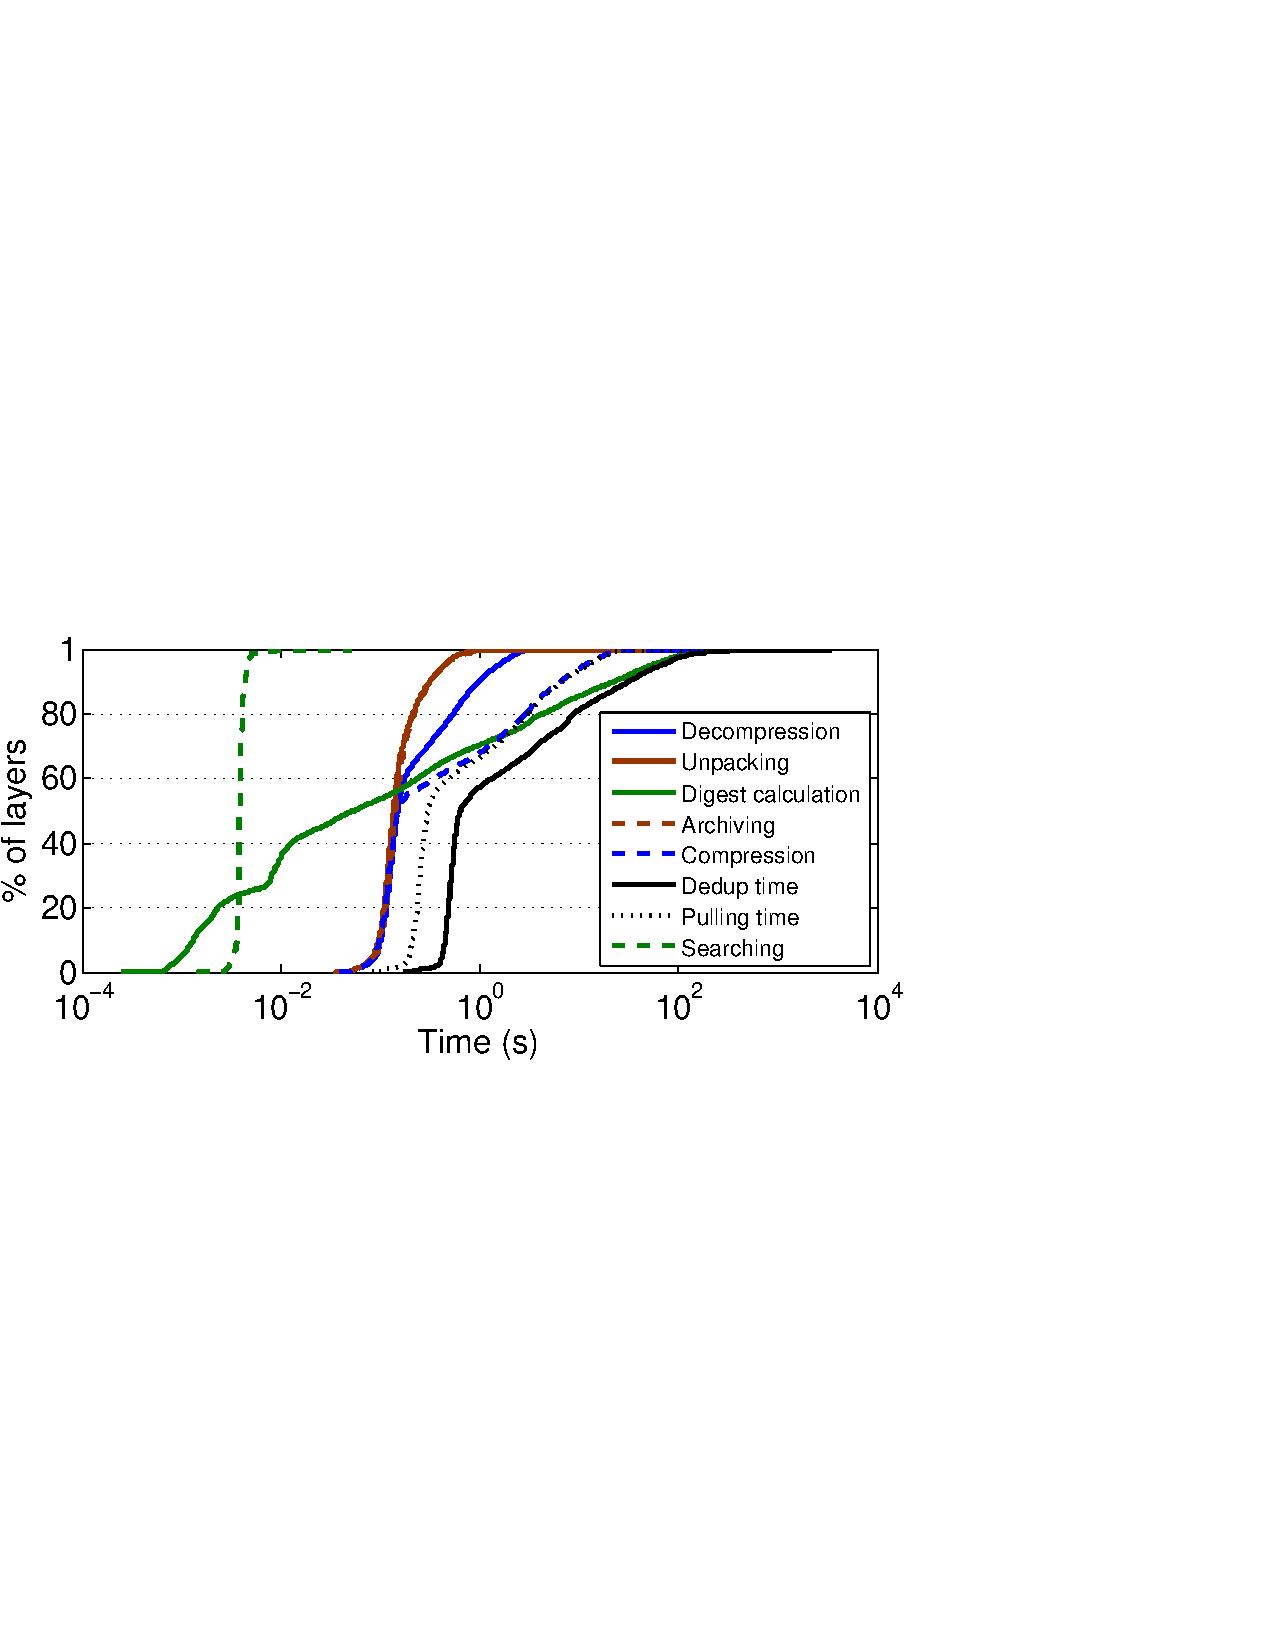
\includegraphics[width=0.5\textwidth]{graphs/res-time.pdf}
	\caption{Off-line file-level deduplication run time.}
	\label{fig:dedup-res}
\end{figure}



%\paragraph{Simulation} 
%
% since dedup process only starts periodically when the
%workload is lower and only cold layers are evolved in dedup process (discussed
%in Section~\ref{subsec:\sysname\}).
%
%\lrcomment{By latency, do you mean the time it takes to perform the dedup? I
%wouldn't call that latency but rather run time or completion time.}
%
%\lrcomment{What exactly was the setup? Where those 60 requests submitted while
%the dedup was running and where they submitted only once or repeatedly?}

\LR{I think the flow in this subsection can be improved. Instead of the ``file-level deduplication
	run time'' paragraph, I would introduce Fig~\ref{fig:dedup-res} at the end of the first paragraph,
	right before ``Push layer latency'' and maybe explain the overal run time there. In the push and pull
	layer latency we can then focus on just the parts of the graph that are related to push and pull.
	This would be a more top-down presentation (which I feel often works better in papers).}
%\NZ{addressed}

\LR{I'm still not sure if we should use simulation or emulation?}
To study the overhead of file-level deduplication, we setup a
one-node Docker registry with 64~GB RAM and 32 Cores.  
%
We wrote around 600 lines of Python code to perform \emph{off-line} file-level deduplication
operations on the layer dataset.
%

\LR{We can remove the following steps once we explained them better
	in 4.0}\NZ{addressed}
% 
%File-level deduplication mainly
%consists of the following steps: 
%layer decompression, 
%file content digest calculation,
%searching \& indexing,
%and storing unique files.
%The unique files are stored in a \textit{file pool}.

Our simulation follows the steps of FLACS as explained above:
First, a layer from the layer dataset is read and copied
to a RAM disk. 
Note that there is no foreground pull or push requests since the simulation is \emph{off-line}.
The layer is then decompressed and 
the digests for each individual file are computed by using MD5 hash function~\cite{MD5}.
\LR{How is the digest computed?}\NZ{addressed}
%
\LR{\emph{emph} should be used instead of \textit{textit} to
	emphasize certain words/parts in the text.}\NZ{addressed}
If the file is not \emph{stored},
we record the \emph{file content address}, which is a
file digest linked to the files' location.
%And we append a \textit{layer-to-file} 
%mapping record to a mapping table. 
%
\LR{This part is confusing. What does ``layer digest to its containing file content
	digest mapping record'' mean? Why is it for each file in a layer and all layers?}
\NZ{addressed}
To map a layer to it's containing files, we create a \emph{layer-to-file} record
%For each file in a layer, 
%a layer digest
%to its containing file content digest mapping record is also created 
and save it
to a \emph{layer-to-file table}.
%
The \emph{layer-to-file table} also
records the file path within each layer associated with each file.
%
Note that we do not consider the latency of storing unique files in our simulation.
%
%Only unique files are maintained in RAM
%disk while the redundant copies are removed.
%
We run \sysname\ for 0.9 Million layers in total and process 60 layers concurrently. 
%
Overall, it took 3.5 days to finish.
%
%
%The overall runtime is about 3.5 days.

\LR{What was the overall runtime for processing 0.9 million layers?}\NZ{addressed}
%
%\alicomment{How are we saving the location
%of each file in the layer? It is not clear from the following sentences.}
%\NZ{addressed}
%
%To improve searching performance, the
%mapping table is stored in Hive database~\cite{xxx}. 
%
%\lrcomment{Why are we using Hive for this? It seems overkill to me, especially
%for such small data. Even at scale, a KeyValue store would probably provide
%better performance than clunky MapReduce-based DB.}
%

\paragraph{Push layer latency}

In our off-line simulation,
\sysname\ does not affect the latency of \emph{push layer} requests
because before performing deduplication, the registry reliably stores
a copy of the layer as is and then sends a response message to the user.
%
Hence, no addition delay will be added to the pushing time. 
%
However, 
if there are intensive push requests while the registry is performing deduplication,
\sysname\ would impact foreground push requests because it incurs 
CPU, memory, and I/O overhead(similar to pull requests).

\paragraph{Pull layer latency} 

For a \emph{pull layer} requests, the registry will first fetch 
all its containing files by consulting the \emph{layer-to-file table}, 
restore the layer archive file by compressing these files, and
then send the compressed layer archive file to the clients.

Figure~\ref{fig:dedup-res} shows a breakdown of the \emph{pull layer}
latency.
%
Note that the \emph{pull layer} latency is the sum of archiving time,
compression time, and searching time and does not include network transfer
time. 
%
\LR{Always add a protected space or a \textbackslash, between a number and its unit.}
\NZ{addressed}
We can see that around 55\% of the layers have a similar compression and archiving
time ranging from from 0.04\,s to 0.15\,s and both operations contribute equally
to pulling latency.
%60\% of compression and archiving time are less than 0.15 s.
%
%While compression has the highest run time 80\% of compression time is less than 2.82~s. 
%
After that, the times diverge and compression times increase faster with an
80\textsuperscript{ts} percentile of 2.82\,s. Hence, compression time makes
up the major portion of the pull latency and becomes a bottleneck.
This is because that the layer size is big\LR{put reason here}
\NZ{I think the layer size is the major reason}.
%
%We see that archiving time and compression contributes equally to pulling
%latency when their run time are lower than 0.15 s while compression time almost
%equals to pulling latency when the compression time is greater than 0.15 s. 
%
To reduce latency, we suggest that fast compression methods should be applied reduce
compression time. As deduplication provides significant storage savings, faster compression
methods with a lower compression ratio are hence feasible.

%\alicomment{Separately mention pull layer requests}
%

\paragraph{File-level deduplication run time}

%and pulling requests for  
%
\LR{This should go under ``Push layer latency''}\NZ{dedup time won't affect the push latency. 
	So we cannot discuss the following latencies in push layer paragraph.}
Figure~\ref{fig:dedup-res} shows the breakdown of run time for each
involved operation: decompression time, unpacking time, file content digest
calculation time, and searching time.
First, among all the operations, we see that searching time is the
smallest. 
%
80\% of searching time is less than 0.004\,s. 
%
The mapping table
maintains 0.98 million layer-to-file digest mapping records. 
%
\LR{Remove the following sentence? 1.7 million records is actually quite
	small so even a single-node DB with one index is enough.}\NZ{addressed}
%
%Consider that more
%than 1.7 million layers are stored in Docker hub and the number is still
%increasing, it's better to choose a fast distributed database to provide high
%searching performance and scalability.
%
%\lrcomment{How does our DB schema look and what are the search queries?}

\LR{This should go under ``Push layer latency''}
Second, we see that digest calculation time spreads over a large range started
from 0.000005 s to 124.7\,s. 
%
This is because digest calculation time mainly
depends on the layer size., \ie the less and smaller files a layer
contains, the faster it is to compute all digests for the layer.
%
%Typically, smaller layers contain a smaller number
%of smaller files, which takes much less time to calculate their digests.
%
%While if the layer is bigger, the digest calculation overhead will be higher. 
%
80\% of digest calculation time is less than 4.21\,s. 
%
Thus, we suggest that multiple-threading is needed to calculate the files'
digests simultaneously; 
%
Fast CPUs as well as more powerful computing nodes are
required to speed up digest calculation.

\LR{This should go under ``Push layer latency''}
\LR{This is pretty much equal to Archiving and Compression times. Does
	that mean in those cases, we're I/O bound?}
\NZ{no, we use RAM disk for storing all layers both in decompressed/compressed format.
	decompresson/compression time depends on layer size, I think.}
Third, the run time for decompression and unpacking have the same distribution
during the lowest response time range started from 0.04\,s to 0.15\,s. 
%
Around 60\% of decompression and unpacking time are less than 0.15\,s. 
%
However, decompression has the highest time than that of unpacking. 
%
80\% of decompression is less than 0.55 s while 80\% of packing time is less than 0.21\,s. 

\LR{This should go at the end of the first part of Section 4.1 and before ``Push layer
	latency''}
Figure~\ref{fig:dedup-res} shows the total time distribution for
file-level deduplication which is the sum of run time for decompression, unpacking,
digest calculation, and searching. 
%
We see that 80\% of file-level dedup time is
less than 9.09\,s per layer.
%
%\lrcomment{Is that per layer or per file or per image?}
%
We also measured the throughput of 60 processes. 
%
Our one-node file-level
deduplication prototype can process about 3\,layers/s. 
%
We suggest to use more
high powerful machines to improve throughput.

%
